%!TEX TS-program = xelatex
%!TEX root = ../../maxwell2018thesis.tex

\chapter[General Methodology]{General Methodology}\label{chap:method}
In Part~\ref{part:context}, we will be exploring how a stopping behaviours vary under different search contexts. In this chapter, we provide an overview of the \emph{general methodology} that we deploy in subsequent contributory chapters of this thesis. The methodology is divided into six main components that are listed below.

\begin{itemize}
    \item{\blueboxbold{Context, Data, Tasks and Retrieval System} This involves the search context, document corpus, topics, tasks and retrieval system used throughout all empirical work in this thesis.}
    \item{\blueboxbold{User Studies} We discuss the general methodology behind two user studies designed to examine how different factors affect stopping behaviours.}
    \item{\blueboxbold{Interaction and Performance Data} We discuss how we extracted key interaction data -- and from these, performance measures.}
    \item{\blueboxbold{Simulations of Interaction} Using the aforementioned interaction data, we outline the methodology behind simulations of interaction that attempt to replicate the user studies.}
    \item{\blueboxbold{Examining Performance} We evaluate the performance of simulated searchers, allowing us to examine what stopping strategies work best under different search contexts.}
    \item{\blueboxbold{Comparing Searchers} Finally, we compare the performance of real-world searchers against simulated counterparts, determining what configurations offer the best approximations to real-world behaviours.}
\end{itemize}

We now discuss each of these different components in depth, highlighting the key decisions that we have made, and discuss supporting literature for our choices. We begin first with a discussion of the retrieval system, document corpus and topics used throughout our remaining contributory chapters.

\section{Context, Data, Tasks and Retrieval System}\label{sec:methodology:collection}
The context for all experiments reported in this thesis is \emph{news search.} As we discuss in this section, we employ an established corpus of news articles and associated topics, with queries issued against the retrieval system described in Section~\ref{sec:methodology:collection:system}.

Given the context of news search, we employ a \emph{simulated work context} with which subjects -- both real-world and simulated -- conform to. As outlined by~\cite{borlund2000simulated_work_tasks} and~\cite{li2013simulated_work_tasks}, simulated work contexts are designed as close as possible to the situations facing real searchers, and thus provide the context that elicit a searcher's interactions with a retrieval system. All search tasks were grounded with a simulated search context. Subjects who participated in user studies were instructed to imagine that they were newspaper reports, and were required to gather articles to write stories about given topics (refer to Section~\ref{sec:methodology:collection:tasks}). These subjects were then asked to identify a number of different articles that they thought were relevant to the given topic.

\subsection{Document Corpus}\label{sec:methodology:collection:corpus}
Under the context of news search, we employed a corpus of newspaper articles. The \emph{\gls{acr:trec} AQUAINT} corpus was selected for all experimentation work in this thesis. The corpus consists of a total of $1,033,461$ news articles (hereon in referred to as \emph{documents)} from the period ranging 1996-2000. All of the documents were collected from three \emph{newswires,} namely: the \emph{Associated Press (AP);} the \emph{New York Times (NYT);} and \emph{Xinhua (XIE).} The AQUAINT corpus was used as it has been extensively used in prior research. Studies include for example:~\cite{collinsthompson2004retrieval_quality, ofoghi2006passage_retrieval, baillie2006query_sampling, azzopardi2008retrievability, kelly2009user_study, azzopardi2013query_cost, maxwell2014temporal_delays, harvey2017searching, yang2017can}; and~\cite{wilkie2017bias}. Basic corpus statistics can be found in the illustration below.

\begin{figure}[h]
    \centering
    \vspace{6mm}
    \resizebox{1\hsize}{!}{
    
\includegraphics{figures/ch6-aquaint-stats.pdf}}
    \vspace{-9mm}
    \label{fig:aquaint_stats}
\end{figure}

\subsection{Retrieval System}\label{sec:methodology:collection:system}
The AQUAINT corpus was then indexed using the \emph{Whoosh~\gls{acr:ir} Toolkit.}\footnote{\emph{Whoosh} can be freely acquired using the \texttt{pip} \emph{Python} package manager -- documentation for Whoosh is available online at \url{http://whoosh.readthedocs.io/en/latest/intro.html}. \urlaccessed{2018-05-18} The corpus was indexed with Whoosh \texttt{2.7.4}.} We applied Porter stemming and removed stopwords as per the 421 term classical stopword list by~\cite{fox1992stopwords}.\footnote{More information on the indexing process can be found in Section~\ref{sec:ir_background:basics:indexing}.} During the indexing process, we also removed documents with duplicate titles. With documents originating from newswires, we found many occurrences of documents with the same title. Document discussing ongoing events were continually revised as new information about said event arose. As such, for documents with duplicate titles, we retained the document with the latest timestamp.

From this process, an index was produced weighing in at $3.8$GB. The index contained a total of $959,678$ indexed documents. The Whoosh~\gls{acr:ir} toolkit was once again used to issue queries against the index. All ranked results for queries were computed with BM25, where $\beta=0.75$ (refer to Section~\ref{sec:ir_background:basics:models:probabilistic}). Terms in all issued queries were implicitly \texttt{AND}ed together to restrict the set of retrieved documents to those that only contained all of the query terms.

\subsection{Topics}\label{sec:methodology:collection:topics}
Five topics were also selected from the 50 provided in the \emph{TREC 2005 Robust Track,} as outlined by~\cite{voorhees2006trec_robust}. These topics were selected based upon evidence from a previous user study (of similar nature) conducted by~\cite{kelly2009user_study}. Evidence showed that the topics offered similar levels of difficulty. The five topics, along with a short description of what constitutes a relevant document, are listed below. These summaries are derived from the TREC topic descriptions that are provided as part of the~\gls{acr:trec} 2005 Robust Track. Figure~\ref{fig:topics} illustrates three examples of topic descriptions.

\begin{figure}[t!]
    \centering
    \resizebox{1\hsize}{!}{
    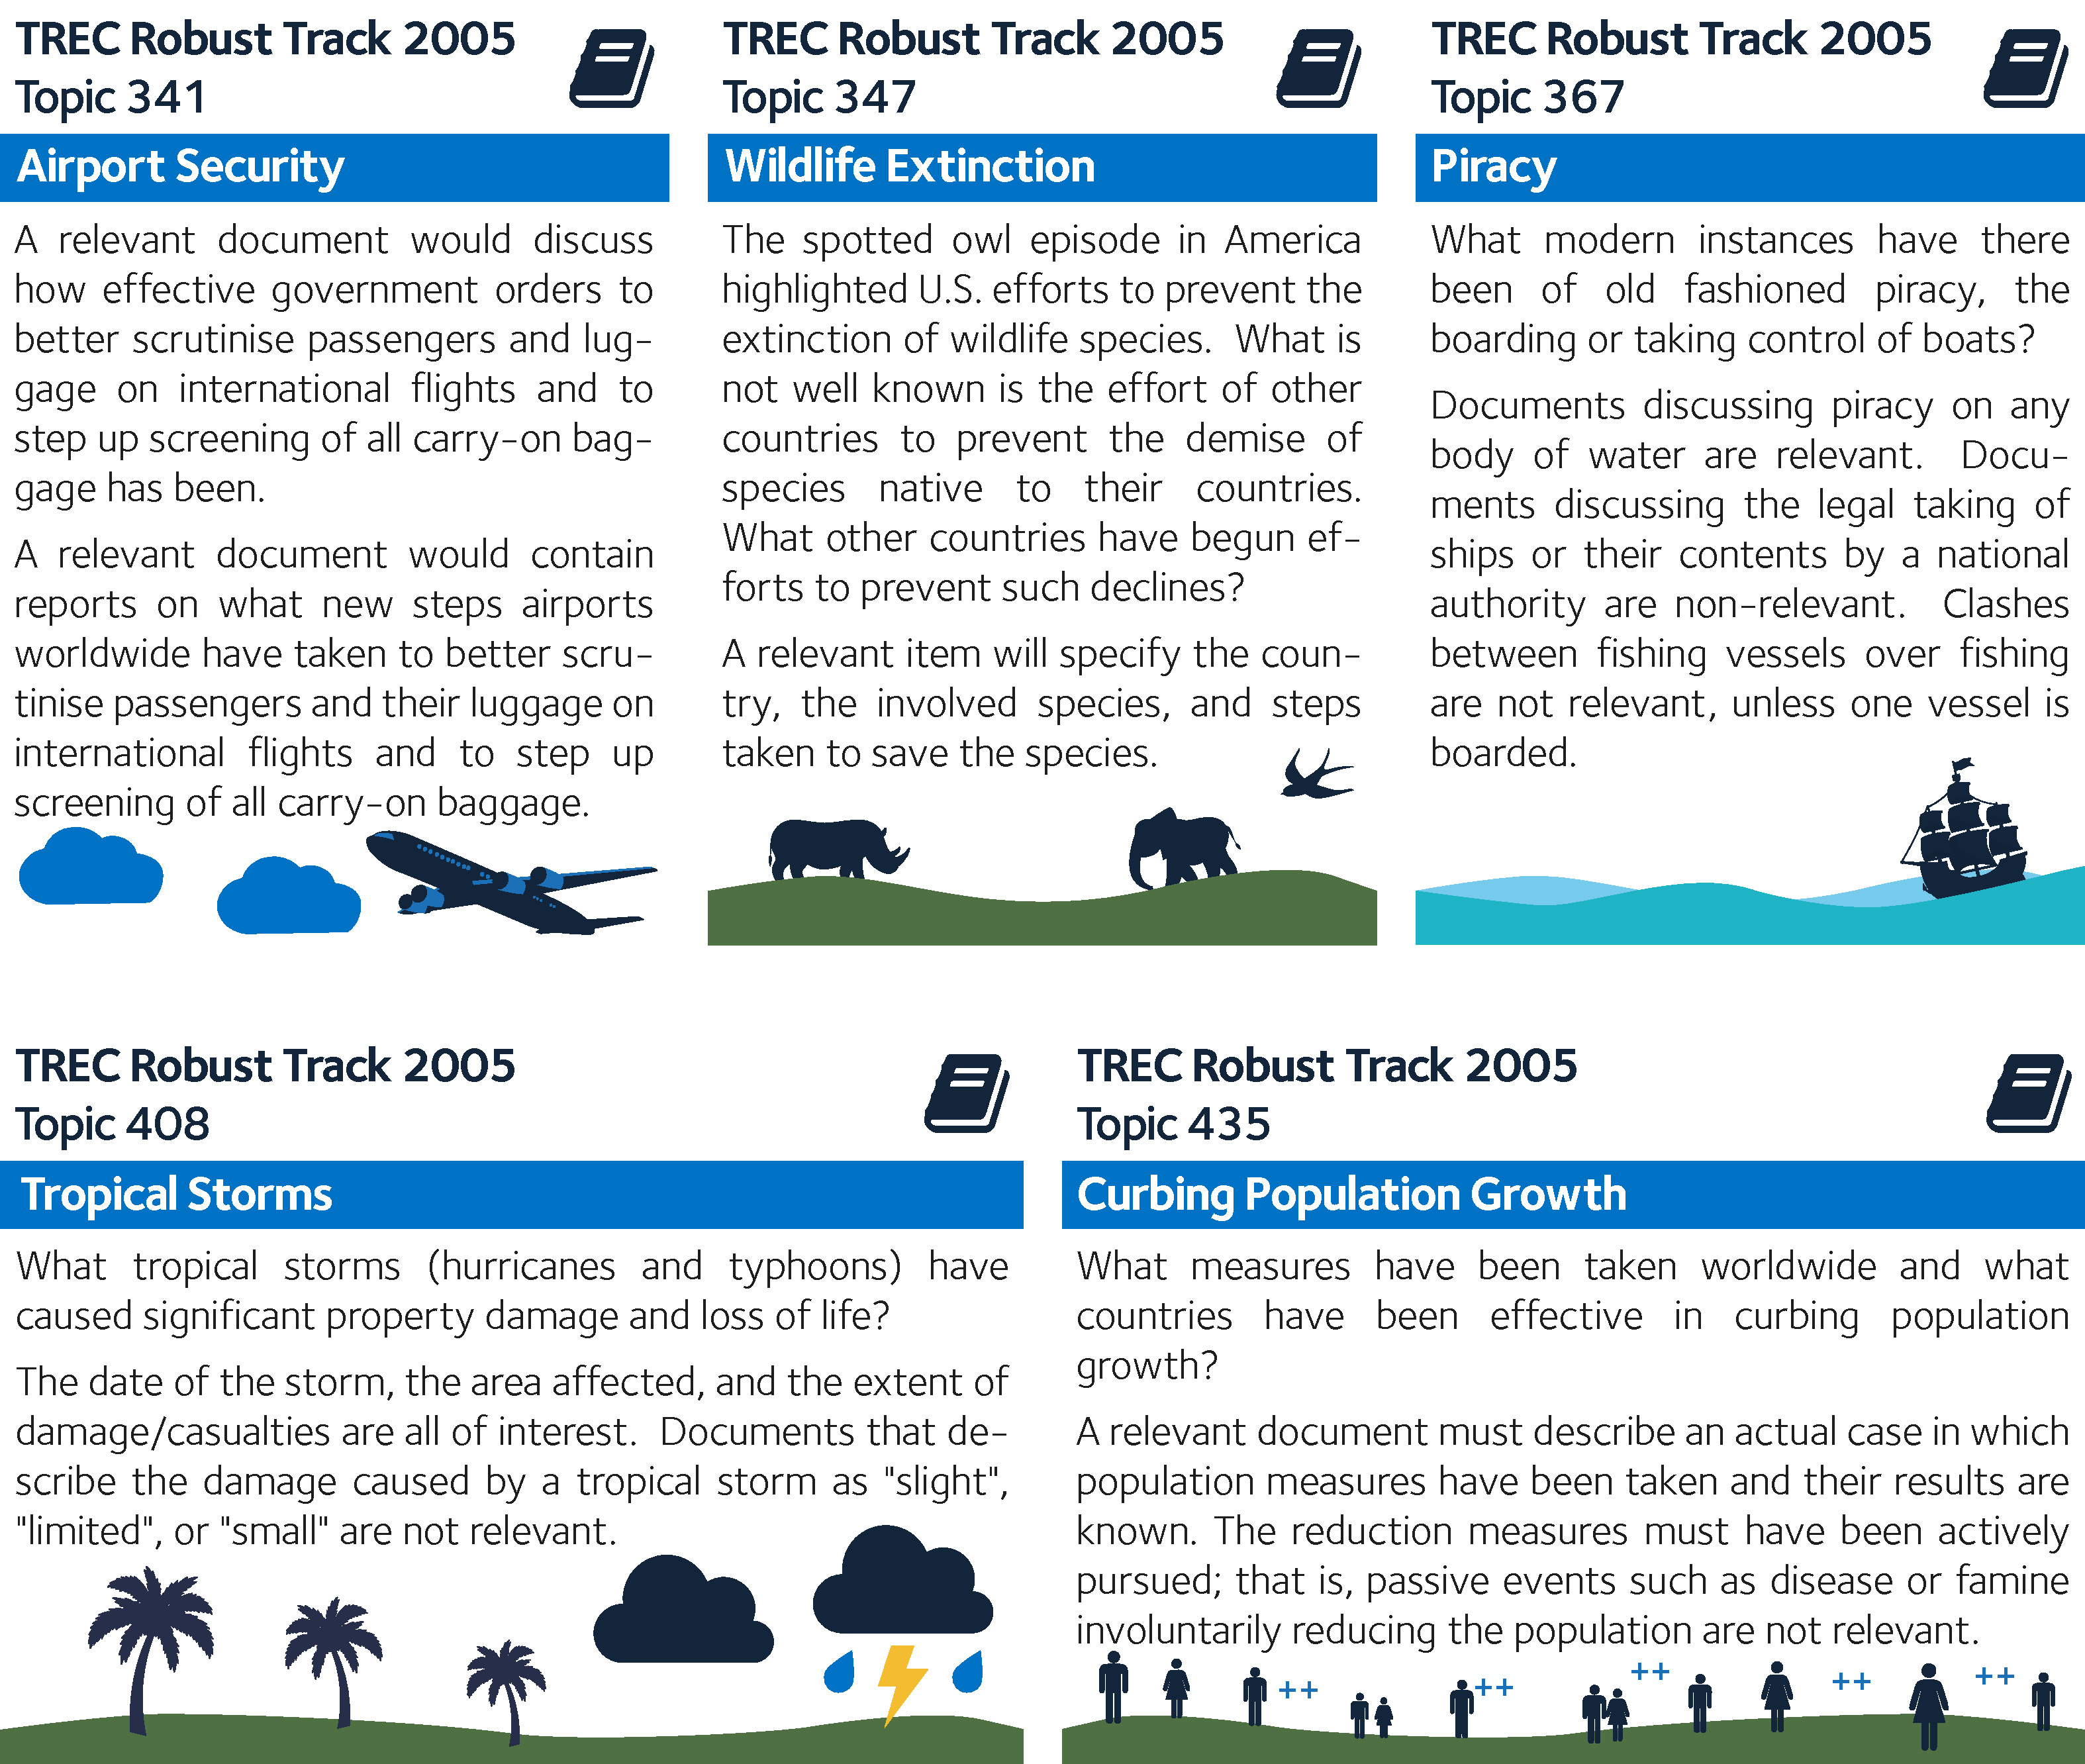
\includegraphics{figures/ch4-topics.pdf}}
    \caption[Examples of TREC Topics]{Three examples of \emph{TREC topic descriptions}. Topics are extracted from the \emph{TREC 2005 Robust Track,} as outlined by~\cite{voorhees2006trec_robust}. Descriptions provide an explanation as to what constitutes a relevant (and often non-relevant) document.}
    \label{fig:topics}
\end{figure}

\begin{itemize}
    
    \item{\blueboxbold{Topic 341 – Airport Security} This topic considers relevant documents as those that discuss additional security measures that were taken by international airports around the world. Relevance is only denoted when a document discusses measures that go beyond the basic passenger and carry-on luggage screening. For example, AQUAINT document \texttt{NYT19980616.0123} discusses \emph{San Francisco International Airport's} attempts at introducing a \emph{robot sniffer,} attempting to look for nitroglycerine in luggage.}
    
    \item{\blueboxbold{Topic 347 – Wildlife Extinction} As the title of the topic suggests, this topic concerns wildlife extinction, and what efforts have been taken by countries \emph{other than} the U.S. to counter the decline in endangered wildlife. Relevant documents explicitly mention the country, the species of animal, and the efforts the state or other governmental agency took to prevent decline in numbers. For example, document \texttt{XIE20000531.0205} discusses the breeding programme undertaken by China to bolster the number of Siberian Tigers in its jurisdiction.}
    
    \item{\blueboxbold{Topic 367 – Piracy} Instances of modern piracy are considered relevant to this topic -- not in the sense of software piracy, but the act of a water going vessel being boarded by individuals wishing to hijack it. Document \texttt{APW19980601.1065} provides an example of this -- the \emph{Petro Ranger}, a large fuel tanker, was boarded by pirates in 1998 in the South China Sea. To be relevant to the topic, the name of the vessel and the body of water it was hijacked on must be mentioned -- those discussing instances of when states intercepted vessels are not relevant.}
    
    \item{\blueboxbold{Topic 408 – Tropical Storms} Documents discussing major tropical storms are to be considered relevant, where the storm is reported to have caused significant damage and a large number of casualties. This is a particularly timely topic for the document corpus considered, as the 1998 hurricane season in the Caribbean has been reported to be one of the most costly -- both in terms of damage caused and lives lost -- in history.\footnote{This is reported by the US \emph{National Oceanic and Atmospheric Administration (NOAA),} as seen at \url{http://www.outlook.noaa.gov/98hurricanes/}. \urlaccessed{2018-05-18}} Document \texttt{APW19980921.1265} for example discusses the effects on Puerto Rico of Hurricane Georges in September 1998, leaving -- at the time of reporting -- three dead, many houses damaged, and thousands homeless.}
    
    \item{\blueboxbold{Topic 435 – Curbing Population Growth} The final topic considers efforts that have been made by countries around the world to control the ever increasing human population. Documents discussing this issue are only relevant to the topic if the results to a case have been made public, and a reduction in population has been actively pursued. The document must mention the country, the As such, events like famines are not relevant. A perhaps well known example of such a phenomenon is the one child policy that was pursued by China in the late 20\textsuperscript{th} century. Document \texttt{NYT19981031.0070} discusses the Chinese government's efforts to curb its expanding population at the time, with sexual education and heavy financial penalties for additional children. These efforts were shown to lead to a reduction in population, although whether this actually occurred is open to debate.}
    
\end{itemize}

For all user studies reported in this thesis, we selected topic \blueboxbold{367} as a \emph{practice topic,} permitting the participating subjects to familiarise themselves with the experimental system used. As such, we do not report any results from interactions that took place with this topic. In the next section, we outline the different search tasks that were undertaken by user study subjects while using these topics.

\section{User Study Methodology}\label{sec:methodology:user}
Using the aforementioned corpus, retrieval system and topics, we now move onto a discussion of the common methodology employed across two user studies. These are detailed in Chapters~\ref{chap:snippets} and~\ref{chap:diversity}. While intricate details of each study's methodology do indeed vary, these are nevertheless common components that we discuss in this section. As a reminder, the two studies examine how a searcher's behaviours, performance perceived user experience varies when:

\begin{itemize}
    \item{the length (and thus quality) of snippets presented in result summaries are varied (Chapter~\ref{chap:snippets}, conducted between July and August, 2016); and}
    
    \item{the overall search goal (time constraints vs. relevancy accruement) and task goal (ad-hoc vs. diversified results) are changed (Chapter~\ref{chap:diversity}, conducted in January, 2018).}
\end{itemize}

Specifically, the methodology used for these studies allowed us to determine how the stopping behaviour of a searcher varies when these conditions are varied. We discuss the specific interfaces and conditions that we trialled in subsequent chapters of this thesis.

Both user studies were undertaken using a custom built experimental framework called \blueboxbold{TREConomics}.\footnote{\treconomics~can be found online at \url{https://github.com/leifos/treconomics}. \urlaccessed{2018-05-15}} The pure-\emph{Python} framework has been developed over a number of years, and allows straightforward deployment of various~\gls{acr:iir}-based studies. It has been successfully deployed in a number of prior works, including those by:~\cite{azzopardi2013query_cost, maxwell2014temporal_delays, kelly2015serp_size, edwards2015query_interface}; and~\cite{crescenzi2016time_constraints}.

% Diversity study -- ethics number 622, Computer and Information Sciences Ethics Committee, University of Strathclyde.

\subsection{Experimental Details and Flow}\label{sec:methodology:user:flow}
Each user study was designed to last for approximately 45-50 minutes, including the completion of requested search tasks and surveys. Both experiments followed a similar structure, where subjects would complete a number of surveys before beginning a search task, and completing a further survey upon completion of the task. These surveys, as discussed in \todo{Section~\ref{sec:csm:methodology:extracting:user},} permitted us to gather a series of usability measures (refer to Section~\ref{sec:ir_background:evaluation:user}) about the perceived experiences of subjects of the various interfaces and conditions.

The basic structure of both user studies was as follows.

\begin{itemize}
    \item{Subjects began by reading the experiment briefing sheet, before agreeing to continue.}
    \item{A demographics survey was then completed.}
    \item{Subjects then attempted the \emph{practice task,} using the practice topic. This allowed subjects to familiarise themselves with the system and its interface.}
    \item{Subjects would then complete the various search tasks set out for them. Each task consisted of three steps:}
    
    \begin{itemize}
        \item{a pre-task survey, capturing a subject's prior knowledge about the topic;}
        \item{the search task itself; and}
        \item{a post-task survey, capturing the subject's experiences regarding searching for information about the topic.}
    \end{itemize}
    
    \item{Upon completion of each search task, subjects would then complete a post-experiment survey, asking general questions about their experience across all the different tasks.}
    \item{Finally, upon completion, subjects would be presented with a results screen, providing a summary of their performance. Performance for each subject was presented on a per-task basis. After this information had been processed, the experiment concluded.}
\end{itemize}

Subjects undertook a total of four search tasks in which interactions and experiences were captured. Including the practice task at the beginning of each experiment, this took the total number of search tasks per subject up to five. Following a \blueboxbold{within-subjects study design}, the four search tasks -- each using a different topic as described in Section~\ref{sec:methodology:collection:topics} -- permitted us to trial each experimental condition/interface. The topics and tasks were assigned to subjects using a Latin-square rotation to minimise ordering effects. A within-subjects design increases the statistical power -- the number of `subjects' is higher than a between-subjects design. Limitations can consider issues such as fatigue. By being considerate of the time spent by subjects searching, fatigue for example could be limited.

\subsection{Experimental Search Interface}\label{sec:methodology:user:interface}
In this section, we discuss the experimental search interface that was used by subjects of the user studies.\footnote{Slight modifications to the search interface were made to the goal-based study, as we discuss in Section~\ref{sec:diversity:users:method}.} The interface would be familiar to anyone who had used a web-based retrieval system, and thus the learning curve for using the interface would most likely be low. Upon commencement of the experiment, the interface would launch in a fixed-size popup window (refer to Section~\ref{sec:methodology:user:crowdsourcing:technical}) of the web browser being used.

The interface consists of three main views, the two most important being shown in Figure~\ref{fig:interfaces}. The views were:

\begin{itemize}
    \item{the~\glsfirst{acr:serp}, presenting the query box and results for an issued query;}
    \item{the \emph{document view,} providing the source text of a documents; and}
    \item{the \emph{saved documents list,} providing a list of the documents that subjects had identified as relevant.}
\end{itemize}

In addition to the three views above, we also provided a \emph{topic view,} which, when requested, would open a further popup window that contained a description of the topic. This was purely to serve as a reminder, as subjects were provided the topic description in full before the search task began.

Common to all views was the inclusion of the blue navigation bar at the top of the popup window. As we discuss further in Section~\ref{sec:methodology:user:crowdsourcing:technical}, this bar was included to provide a series of different navigational links, such as, when on the document view page, a link to return to the originating~\gls{acr:serp}. Where applicable, we also provided a link for the subject to end the search task, if he or she felt that they had satisfied the criteria for the task.

\begin{figure}[t!]
    \centering
    \resizebox{1\hsize}{!}{
    
\includegraphics[width=1\textwidth]{figures/ch6-interfaces.png}}
    \caption[Example screenshots of the experimental interfaces]{Example screenshots of the basic search interface used as part of \treconomics. On the left is a screenshot of typical experimental~\gls{acr:serp} for the query \texttt{wildlife extinction}. The right shows the document view, showing the option for subjects to \texttt{Save} a document that they consider relevant to the given topic.}
    \label{fig:interfaces}
\end{figure}

\subsubsection{The~\gls{acr:serp}}\label{sec:methodology:user:interface:serp}
As can be observed from the left screenshot in Figure~\ref{fig:interfaces}, the~\gls{acr:serp} does not look all that different from a~\gls{acr:serp} on a contemporary web search engine -- sans right rail components, as we discussed previously in Section~\ref{sec:ir_background:basics}. The experimental~\gls{acr:serp} provides at the top the \emph{query box,} allowing subjects to enter their query term(s), and a button to submit their query. The \texttt{ENTER} key could also be used to submit a query.

Once submitted, results are displayed underneath the query box. The issued query is provided, along with an approximation of how many pages of results are provided to the searcher for the given query. This hints that pagination is utilised -- with 10 results per page shown. At the bottom of each~\gls{acr:serp} are links that allow the searcher to move to the previous and next page of results.

\begin{figure}[h]
    \centering
    \vspace{4mm}
    \resizebox{1\hsize}{!}{
    
\includegraphics{figures/ch6-buttons.pdf}}
    \label{fig:serp_buttons}
    \vspace{-5mm}
\end{figure}

Result summaries were shown as discussed in Section~\ref{sec:ir_background:user:iir:serp}. The title, the source, and any snippet text were all provided. Given that the experiments were based upon news search, the source is the name of the newswire from which the document originates. The title was also hyperlinked.

\begin{figure}[h]
    \centering
    \vspace{0mm}
    \resizebox{1\hsize}{!}{
    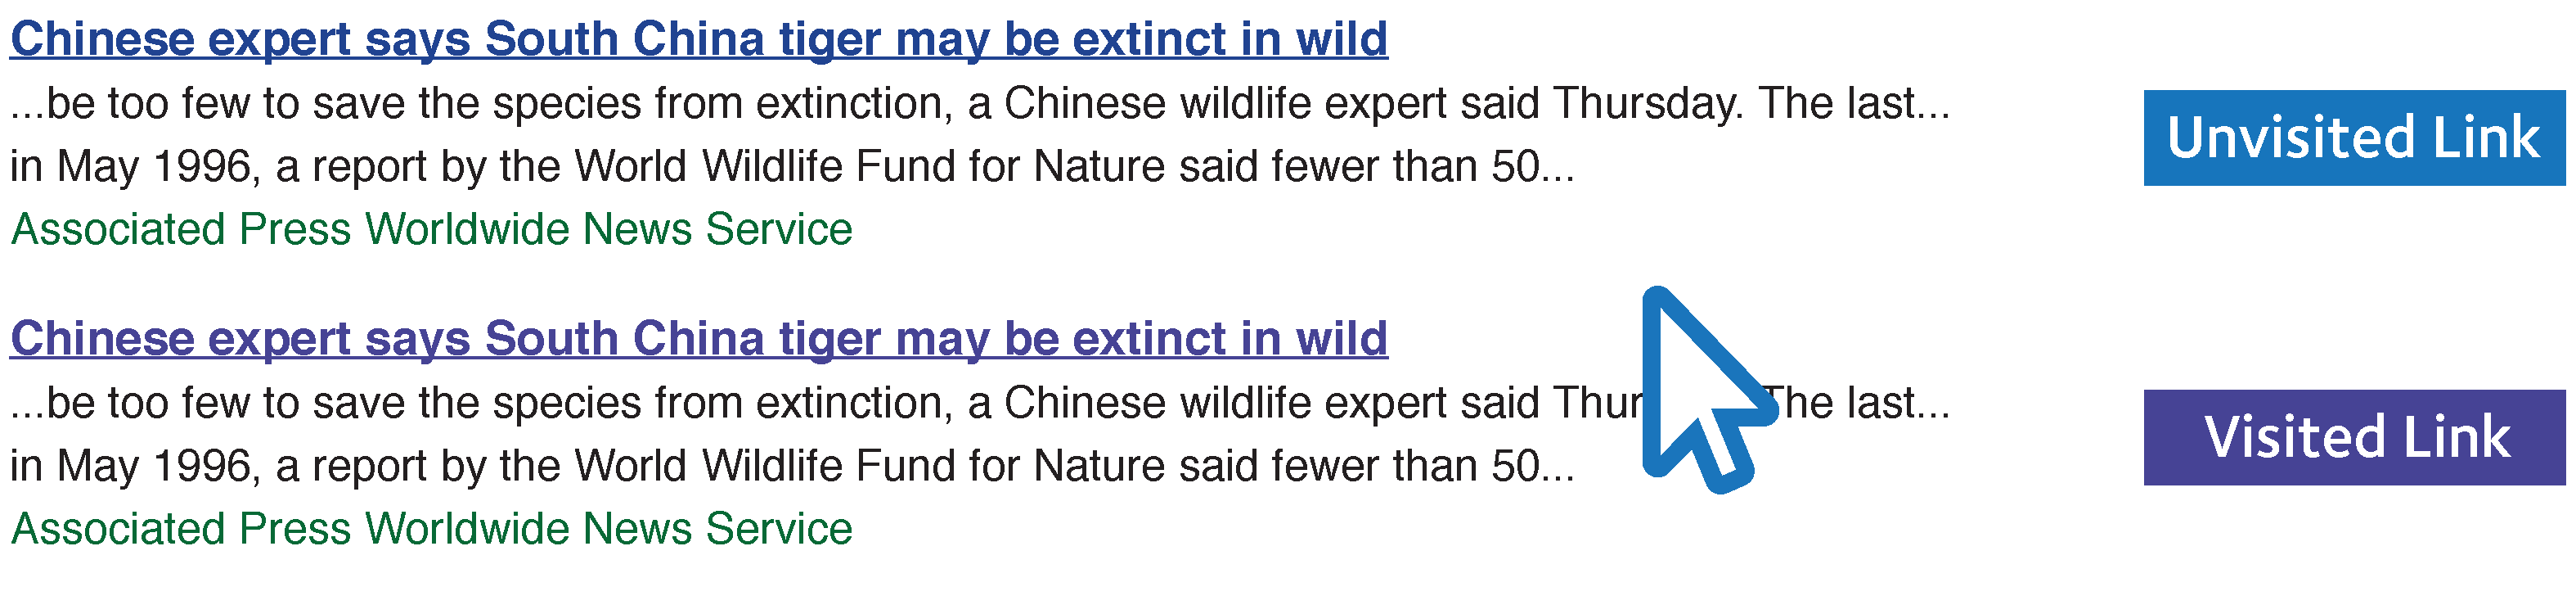
\includegraphics{figures/ch6-links.pdf}}
    \label{fig:serp_links}
    \vspace{-13mm}
\end{figure}

When a subject clicked on the link, he or she would then be taken to the document view (discussed below), displaying the associated document in its entirety. Standard hyperlink colours were employed -- blue for unvisited, and purple for visited. Examples of these link colours are shown above.

\subsubsection{The Document View}\label{sec:methodology:user:interface:document}
The right screenshot in Figure~\ref{fig:interfaces} illustrates the document view. The view provides the title, the document source (newswire), the date at which the document was created, and the full text of said document. On the right rail of the page, subjects were provided with two buttons -- one to return them to the originating~\gls{acr:serp}, or another to \emph{save} the document. The act of saving a document is a crucial component to both studies we discuss in this thesis. It provided us with a mechanism to determine what documents subjects thought were relevant to the given topics. This mechanism for instance also provided us with a means to calculate a subject's performance.

\subsubsection{The Saved Documents View}\label{sec:methodology:user:interface:saved}
The third key view, as mentioned above, allowed subjects to view a list of documents that they had previously saved as relevant to the given topic. This list of documents also provided buttons, allowing subjects to change their decisions as to what constituted as a relevant document. We provided this functionality as~\gls{acr:iir} is inherently an interactive process -- a searcher \emph{learns} and develops their mental model of the given information need as more information is presented to them~\citep{ingwersen2005theturn}.

\subsection{Capturing Interactions and Survey Responses}\label{sec:methodology:user:capturing}
In addition to the interface, the \treconomics~framework provided extensive logging capabilities to capture a variety of different events triggered by subjects as they performed search tasks. This resulted in the generation of an experiment \emph{log file,} capturing the date, time, searcher and topic for each event that was logged. Figure~\ref{fig:log} provides an anonymised excerpt from the interaction log of the user study presented in Chapter~\ref{chap:snippets}.

The figure illustrates the different actions that were logged from when a searcher begins interactions with the query box (\texttt{QUERY\_FOCUS}), to issuing a query (\texttt{QUERY\_ISSUED}, complete with the terms of the query), to clicking a document (\texttt{DOC\_CLICKED}), and, finally, to saving the document (or considering it relevant to the given topic, \texttt{DOC\_MARKED\_RELEVANT}). A detailed discussion of the different behavioural measures that we examined from the interaction log are detailed in Section~\ref{sec:methodology:extracting}.

\begin{figure}[t!]
    \centering
    \resizebox{1\hsize}{!}{
    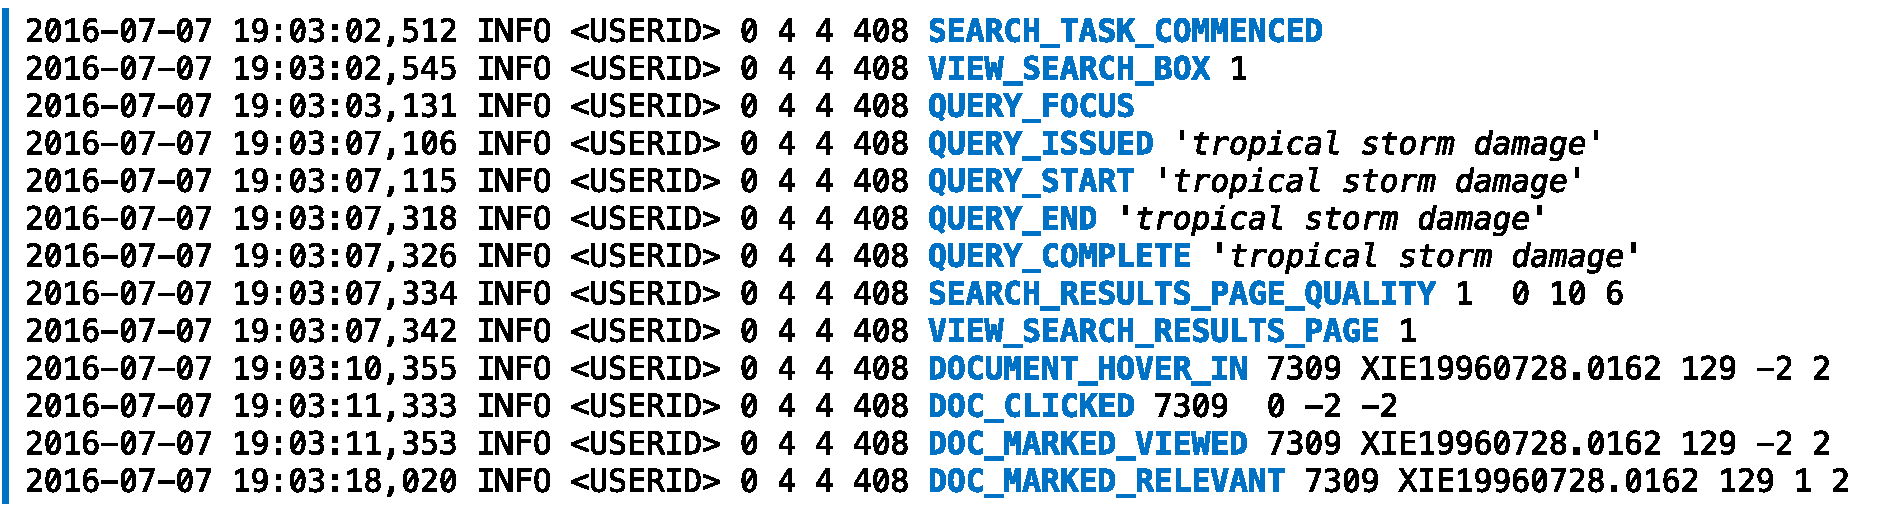
\includegraphics{figures/ch6-log.pdf}}
    \caption[Experiment log file excerpt]{An excerpt from the interaction log of the user study detailed in Chapter~\ref{chap:snippets}. A sequence of interactions are shown that were logged by the \treconomics~framework.}
    \label{fig:log}
\end{figure}

The \treconomics~framework also saved the responses from surveys as completed by the subjects of each study. These were saved to a separate~\gls{acr:rdbms}, with a number of scripts subsequently created to extract and analyse the saved responses.

\subsection{Crowdsourcing Considerations}\label{sec:methodology:user:crowdsourcing}
An important factor in planning any user study is the economics of collecting input from subjects. \emph{Where do the subjects come from? How do we recruit them?} A traditional, lab-based study as discussed in Section~\ref{sec:ir_background:user} typically involves a significant investment in time and monetary cost from the researchers conducting the experiment~\citep{spool2001testing}. For both user studies previously detailed, we employed a \emph{crowdsourced} approach to our experimentation. Crowdsourcing is the practice of obtaining input into a task by enlisting the services of a number of people, recruited over the Internet.

As highlighted by~\cite{zuccon2013crowdsourcing_comparisons}, crowdsourcing provides an alternative means for capturing user interactions and search behaviours. Greater volumes of data can be obtained from more heterogeneous workers at a lower cost -- all within a shorter timeframe. Of course, pitfalls of a crowdsourced approach include the possibility of workers completing tasks as efficiently -- but not effectively -- as possible, or submitting their tasks without performing the requested operations~\citep{feild2010turkers}.

Despite these issues, it has been shown that there is little difference in the quality between crowdsourced and lab-based studies~\citep{kely2011user_study, zuccon2013crowdsourcing_comparisons}. Nevertheless, quality control is a major component of a well-executed crowdsourced experiment, with examples in a similar research area including work by:~\cite{kazai2011crowdsourced, crescenzi2013crowdsourced}; and~\cite{bota2016information_cards}.

Using crowdsourcing for the two user studies, we detail in the remainder of this section the precautions that were taken during, discussing both the requirements for the subjects and their technical setup -- as well as a discussion of the crowdsourcing platform used.

\subsubsection{Platform Details}\label{sec:methodology:user:crowdsourcing:platform}
Both studies were run over the~\glsfirst{acr:mturk} platform. Workers\footnote{In this section, a \emph{worker} refers to an individual undertaking the experiment on the MTurk platform. This term is considered interchangeable with a \emph{subject.}} from the platform each performed a single task (or, to use MTurk language, a \emph{Human Intelligence Task (HIT)}), with a single HIT corresponding to the entire experiment. This is in contrast to many other crowdsourced studies, where workers would typically undertake small -- typically decision-based -- HIT transactions.

\subsubsection{Subject Requirements}\label{sec:methodology:user:crowdsourcing:subjects}
Due to the expected length that workers would take to complete the two studies\footnote{Note that two different sets of workers were used -- the studies were run at different times.}, workers who completed the study in full were reimbursed for their time with US\$9 -- greater than the hourly minimum wage set by the US federal government. Workers interested in undertaking each of the two studies were required to meet a certain minimum set of criteria to be eligible to participate. We required that workers were:

\begin{itemize}
    \item{from the U.S.;}
    \item{native English speakers;}
    \item{possessed a HIT acceptance rate of at least 95\%; and}
    \item{had at least had 1000 prior HITs approved.}
\end{itemize}

Requiring a high HIT acceptance rate reduced the likelihood of recruiting workers who would not complete the study in a satisfactory manner. Recruits were forewarned about the length of the HIT, providing them with a chance to abandon the experiment if they felt the expected time was too long.

\subsubsection{Technical Requirements}\label{sec:methodology:user:crowdsourcing:technical}
Given worker limitations, we also enforced a number of technical constraints. Workers attempting each experiment were required to have a sufficiently large computer screen to display the experimental interface without having to resort to excessive scrolling, and ensured a consistent number of result summaries would be present on different worker's screens. As such, we imposed a minimum display resolution of $1024x768$ for both studies. 

Conducted through a web browser, we wanted to ensure that only the controls provided by the experimental apparatus were used, meaning that the popup window that we highlighted in Section~\ref{sec:methodology:user:interface} had all other browser controls disabled to the best of our ability (i.e. browser history navigation, etc.). The experimental system was tested on several major web browsers (including \emph{Google Chrome, Mozilla Firefox,} \emph{Apple Safari} and \emph{Microsoft Edge)}, across different operating systems (including \emph{Microsoft Windows,} \emph{Apple macOS} and several \emph{Linux} distributions, focusing on \emph{Ubuntu)}. This gave us confidence that a similar experience would be had across different system configurations.

\section{Extracting User Study Data}\label{sec:methodology:extracting}
As discussed in Section~\ref{sec:methodology:user:capturing}, the \treconomics~framework provided the necessary infrastructure for us to log the various interactions and capture survey responses from each individual subject across the two user studies trialled. In this section, we provide details on the different aspects that we subsequently used to evaluate searcher behaviours, performance and user experience. Figure~\ref{fig:evaluation_methodology} provides a graphical illustration of how we split the various aspects we consider into four distinct categories.

The first three categories can be extracted directly from the interaction log that recorded different interactions by each subject as they progressed through the experiment. The categories we considered are listed below.

\begin{itemize}
    
    \item{\blueboxbold{Behavioural Measures} capture the broad interactions that take place, such as the number of documents that a searcher examined in detail.}
    \item{\blueboxbold{Performance} measures could then be extrapolated, with aid of~\gls{acr:trec} QREL relevance judgements, to ascertain the performance of subjects.}
    \item{\blueboxbold{Time-Based} measures can also be derived from directly examining the interaction log, measuring the time spent between different logged interactions.}
    
\end{itemize}

In addition to these categories, we also considered a number of \blueboxbold{user experience} measures that were derived from a series of surveys. As highlighted in Section~\ref{sec:methodology:user:flow}, surveys were presented to subjects at a number of different stages throughout the experiment. In conjunction with the three log-based categories defined above, the user experience measures could be used to complement the empirical evidence to see whether the interactions of subjects actually correlated with their perceived experiences.

In all, the interactions -- including aspects such as clicks, and time-based measures, were used as a \emph{grounding} for our subsequent user simulations of interaction. \todo{How we grounded these simulations is discussed in Section~\ref{chap:csm:method:simulation}}.

\begin{figure}[t!]
    \centering
    \resizebox{1\hsize}{!}{
    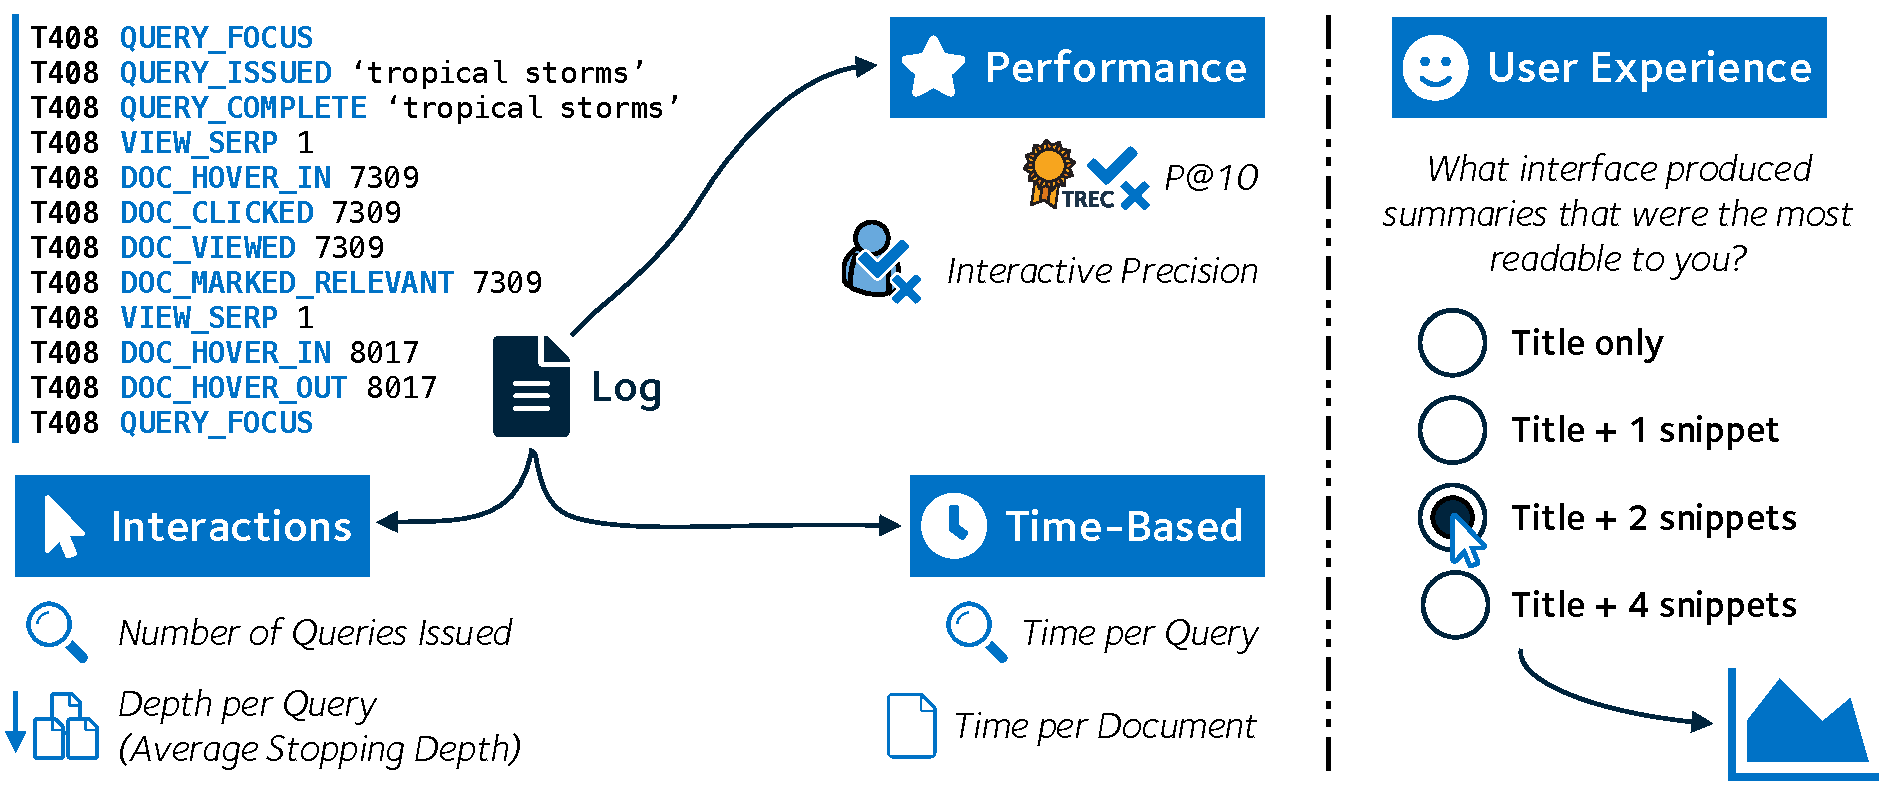
\includegraphics{figures/ch4-evaluation.pdf}}
    \caption[Examples of evaluation measures]{An illustration of the different types of measures that are captured, and from what sources. Interaction, time-based and performance measures are derived from the user study experiment log (with~\gls{acr:trec} QRELs used in conjunction with the interaction log to compute a subject's performance). User experience metrics are collated from a number of different surveys. Refer to Section~\ref{sec:methodology:extracting} for more information.}
    \label{fig:evaluation_methodology}
\end{figure}

\subsection{Behavioural Measures}
Recorded solely from interaction log data, the basic interactions covered a large proportion of the aspects we considered in our analyses. They key behavioural measures we examined are listed below.

\begin{itemize}
    \item{\blueboxbold{Queries} We considered the number of queries that had been issued.}
    \item{\blueboxbold{Documents} The number of documents that were examined (viewed).}
    \item{\blueboxbold{\glsplural{acr:serp}} The number of~\glsplural{acr:serp} that were examined.}
    \item{\blueboxbold{Examination Depth} The depth to which subjects clicked on (and hovered over) result summaries on the associated~\glsplural{acr:serp}.}
\end{itemize}

From these measures, we could then ascertain whether searcher behaviour varied when a certain condition or interface was changed -- allowing us to address questions such as \emph{whether snippet length affects the depth to which searchers examine content?} To compute depths, click and hover depths were used -- we however only report click depths in subsequent contributory chapters. The reasoning for this is \todo{discussed in Section~\ref{sec:csm:methodology:extracting:time} below.} These measures were computed over each query issued by the different subjects.

% -- we could then take an average for each subject. We could go even further, too -- averaging over each topic, interface or condition as required to observe any notable trends in behavioural changes.

\subsection{Time-Based Measures}\label{sec:methodology:extracting:time}
As discussed in Section~\ref{sec:methodology:user:capturing} -- and also illustrated in Figure~\ref{fig:log} on page~\pageref{fig:log}, each logged interaction was saved with a timestamp which allowed us to determine when each event occurred.\footnote{Timestamps were saved to the nearest thousandth of a second, as per the specification of the standard Python logging framework -- refer to \url{https://docs.python.org/2/howto/logging-cookbook.html} \urlaccessed{2018-05-29} for an example of the framework in action.} With these timestamps, we could then measure the time between two associated events, thus yielding the time taken to perform a given activity. We considered five key time-based measures across both user studies that we enumerate below.

\begin{itemize}
    \item{\blueboxbold{Queries} The time spent issuing queries to the retrieval system.}
    \item{\blueboxbold{\gls{acr:serp} Content} The time spent examining content on~\glsplural{acr:serp}.}
    \item{\blueboxbold{Result Summaries} The time spent examining individual result summaries.}
    \item{\blueboxbold{Documents} The time spent examining individual documents.}
\end{itemize}

The summation of all of the above yielded the \blueboxbold{total session time}, a measure that we also considered. It should be noted that in this thesis \blueboxbold{we report all durations in seconds}.

A number of different approximations were required when measuring each of the above. For example, we approximated the query time as the time between the \texttt{QUERY\_FOCUS} to \texttt{QUERY\_ISSUED} events. Subjects may have spent longer considering what terms to enter; our logging tools were not capable of capturing this additional time, only the time spent interacting with the search box.

Following a simple linear model, we could also approximate the total time spent on a~\gls{acr:serp} could be computed as:

\begin{equation*}
    t_{SERP} = t_{0} + (|summaries| * t_{summary}),
\end{equation*}

\noindent
where: $t_{0}$ denotes the initial time spent before summary interaction occurred; $|summaries|$ denotes the number of result summaries interacted with; and $t_{summary}$ denotes the time taken for each result summary to be examined. The time per result summary was approximated by dividing by the click depth reached on a given~\gls{acr:serp}. This was originally computed by summing up the time spent hovering over results with the subject's mouse cursor, as this was shown in prior studies to correlate strongly with the user's gaze on the screen~\citep{chen2001mouse_cursor, smucker2014judging_relevance_movements}. However, issues with network latency meant that several of the hover events were logged in the incorrect order, making such an approach unreliable. Using the click depth and total~\gls{acr:serp} time provided us with an approximation with which to work with. However, the approximation also makes an assumption that subjects examined each result summary on a~\gls{acr:serp} up to a particular depth, for an equal period of time. This was sufficient for the work in our study to ascertain whether or not a variation in the task goal or presentation of results affected search depths.

\subsection{Performance Measures}\label{sec:methodology:extracting:performance}
In conjunction with behavioural and time-based measures, we were also able to extract a number of different performance measures from the interaction logs.\footnote{Some measures were computed with the \texttt{trec\_eval} evaluation tool, discussed in Section~\ref{sec:ir_background:basics:cranfield:trec}.} Key performance measures that we captured included:

\begin{itemize}
    \item{\blueboxbold{query performance}, measured with $P@10$; and}
    \item{\blueboxbold{interactive precision and recall} (as discussed in Section~\ref{sec:ir_background:evaluation:user:ipr}), including:}
    
    \begin{itemize}
        \item{the number of documents saved (identified as relevant); and}
        \item{the number of those documents that were~\gls{acr:trec} relevant (and vice-versa).}
    \end{itemize}
\end{itemize}

\blueboxheader{Grounding Subsequent Experiments} With behavioural measures and time-based measures in particular, these could be then used to \emph{ground} subsequent simulations of interaction. \todo{Refer to Section~\ref{chap:csm:method:simulation:grounding}} for further information on how this was achieved. The above measures were however sufficient for analysing how searcher behaviour changed.

\subsection{Demographics and User Experience Surveys}\label{sec:methodology:extracting:user}
A number of surveys were also filled out by subjects. These captured different information about each searcher's individual search experiences. While there are similarities between what is asked (refer to Sections~\ref{sec:snippets:method} and~\ref{sec:diversity:users:diversifying} for further details), we in this section provide a high-level overview of the different surveys, before examining questions that were common between the two. We break these overviews into three sections, in the order of the experimental flow detailed in Section~\ref{sec:methodology:user:flow} -- demographics, pre- and post-task surveys, and post-experiment surveys.

\subsubsection{Demographics}
Details in keeping with general demographics were attained about the different subjects from this survey. These included the following basic demographic questions:

\begin{itemize}
    \item{the subject's age and gender;}
    \item{their present occupation; and}
    \item{their highest level of professional qualification (e.g. high school, Honours, MSc or PhD).}
\end{itemize}

In addition to these basic questions, we also asked several questions pertaining to their perceived search proficiency. Questions included:

\begin{itemize}
    \item{how often they searched for information;}
    \item{how often they search for news articles (being a news-based experiment);}
    \item{what pointing device they were using (i.e. mouse, trackpad); and}
    \item{their preferred general purpose web search engine.}
\end{itemize}

Considering that both experiments considered the news searching domain, we asked each subject how often they searched for news articles online.

\subsubsection{Pre-Task}
Between both user studies, we asked the same questions within the pre-task survey. Subjects were provided with a short description of their search task and a topic description, providing their information need for said task. After examining the topic description, subjects were then queried on the following:

\begin{itemize}
    \item{how well they knew about the topic prior to this study;}
    \item{how relevant the topic was to their life;}
    \item{how interested they were to learn more about the topic;}
    \item{whether they had searched for information related to the topic before; and}
    \item{how difficult they felt it would be to search for information on the topic before commencing.}
\end{itemize}

Responses were provided on a seven-point scale, providing the option for neutrality between the two extremes -- extremes being \emph{nothing/not at all/very difficult} to \emph{lots/very much/very easy.} Responses to these questions helped us gauge the perceived difficulty of the task, and ascertain how much background knowledge could potentially affect results.

\subsubsection{Post-Task and Post-Experiment}
Post-task and post-experiment surveys were unique to each of the two user studies. Sections~\ref{sec:snippets:method} and~\ref{sec:diversity:users:diversifying} provide further information on what questions were asked. However, the post-task surveys focused on how well the subjects thought they (and the retrieval system, under the given condition and/or interface) performed during the search task. Post-task surveys considered the experiment as a whole, asking questions about what condition and/or interface the subjects preferred, or performed more to their liking, for example.

\section{Simulating Searcher Behaviours}\label{sec:method:simulation}
With the general layout and components of the two user studies explained, we now consider how we \emph{simulated searcher behaviours.} The simulation of interaction provides a low-cost means for exploring a variety of different searcher strategies and configurations~\citep{azzopardi2010workshop}. In this section, we provide an overview of the general aspects of the \blueboxbold{stochastically-based} searcher simulations that we discuss the results of in subsequent chapters of this thesis. Specifically, we discuss in this section:

\begin{itemize}
    \item{how our simulations were \emph{grounded;} and}
    \item{how we instantiated the different components of the~\gls{acr:csm} defined in Chapter~\ref{chap:csm} for our simulation experiments.}
\end{itemize}

We conclude the chapter with a discussion as to how we evaluate the results from our simulations, allowing us to determine what stopping strategies offer the best overall performance and approximations of real-world searcher behaviours. This is done in consideration of the two user studies discussed in Chapters~\ref{chap:snippets} and~\ref{chap:diversity}. By grounding our simulations with data derived from the two aforementioned user studies, we can then obtain an insight into how searcher stopping behaviours vary under different contexts.

\blueboxheader{The Mean Searcher} Comparisons between simulations and real-world searcher approximations are made between the \emph{average} behaviours observed. This average behaviour is considered across each of the different experimental interfaces and conditions that we trial across the two user studies, discussed in Chapters~\ref{chap:snippets} and~\ref{chap:diversity}. This consideration:

\begin{itemize}
    \item{simplifies and reduces the number of simulations that are required to be run; and}
    \item{provides a simple overview of how stopping behaviour varies across each interface and condition, rather than across each individual searcher.}
\end{itemize}

\blueboxheader{Considering Stochastic Simulations} We consider a series of different \emph{stochastically-based} simulations that attempt to mimic searcher behaviours. Currently, a majority of research that considers the simulation of interaction are also stochastic in nature, utilising probabilistic models. For example,~\cite{carterette2011effectiveness_evaluation} simulated the interaction of users for the purposes of evaluation through a dynamic test collection. While not explicitly stated, the underlying model of their simulations followed a similar process to the~\gls{acr:csm} as described in Chapter~\ref{chap:csm}, and were instantiated with probabilistic components.~\cite{baskaya2013behavioural_factors}, as discussed in Section~\ref{sec:ir_background:user:models}, developed a Markov-based model of the search process, with changes in state determined by a series of different probabilities. A similar, probabilistic browsing model was also proposed by~\cite{yilmaz2010browsing_utility}. These models considered probabilistically determining, for instance, the attractiveness of a result summary to the given information need -- something that we also utilise. \todo{We discuss this further in Section~\ref{chap:csm:method:simulation:grounding:judgements}.}

\subsection{The SimIIR Framework}\label{sec:method:simulation:simiir}
All simulations that were run as part of this thesis were performed using the \simiir~framework, a custom built framework for the simulation of interaction within the wider~\gls{acr:iir} process~\citep{maxwell2016simiir}.\footnote{\simiir~can be accessed at \url{https://github.com/leifos/simiir}. \urlaccessed{2018-05-29}} The framework consists of a number of individual \emph{components,} each which must be instantiated to yield a \emph{simulation.} In this section, we briefly outline the different components of the framework, discussing the need for each. Each of these components can be mapped to one of the individual decision points and/or activities of the \gls{acr:csm}, as outlined in Section~\ref{sec:csm:flow} on page~\pageref{sec:csm:flow}.

A \emph{simulation} within the \simiir~framework consists of the following main components.

\begin{itemize}
    \item{\blueboxbold{Topics} One or more topic(s) can be supplied, each consisting of a title and topic description (i.e. the~\gls{acr:trec} topic descriptions).}
    \item{\blueboxbold{Retrieval System} An interface is provided to retrieval system that is to be used with the experiment. In the case of this thesis, this links back to the setup described in Section~\ref{sec:methodology:collection:system}.}
    \item{\blueboxbold{Output Controller} This component is responsible for generating the output files that can be fed into evaluation programs such as \texttt{trec\_eval}, as outlined in Section~\ref{sec:ir_background:paradigms:trec}.}
\end{itemize}

Simulations also consist of one or more \blueboxbold{simulated searchers}, which attempt to complete a given search task, having been instantiated with differing constraints. A simulation is therefore in essence loosely associated with the concept of a real-world \emph{user study.} Each individual searcher -- that can be likened to an individual subject of a user study -- consists of additional components that \emph{describe their behaviours.}

\begin{itemize}
    \item{\blueboxbold{Querying Strategy} The querying strategy determines how queries are generated from topic descriptions, and subsequently selected.}
    \item{\blueboxbold{\gls{acr:serp} Decision Maker} This decision maker determines where a searcher should \emph{enter} a~\gls{acr:serp} and begin to examine individual result summaries, or abandon the~\gls{acr:serp} and issue a subsequent query.}
    \item{\blueboxbold{Classifier/Decision Maker} These components are responsible for judging the attractiveness and relevancy of result summaries and documents respectively.}
    \item{\blueboxbold{Result Summary Level Stopping Strategy} This component, instantiated using one of the stopping strategies outlined in Chapter~\ref{chap:strategies}, determines the point at which a simulated searcher will stop interacting with a ranked list of results.}
    \item{\blueboxbold{Logger} The logger component is responsible for providing \emph{interaction costs} for particular interactions (e.g. issuing a query), keeping track of the combined session time, and determining whether the overall search session goal, time limit -- or other session level stopping constraint -- has been met.}
    \item{\blueboxbold{Search Context} This component can be considered as a basic representation of a searcher's brain, keeping track of the different result summaries and documents that have been examined, prior queries that have been issued, and what documents have been identified as relevant.}
\end{itemize}

All the above components are underpinned by a \blueboxbold{searcher model} component, providing a flow of interactions to the search process undertaken by simulated searchers. In all simulations reported in this thesis, this consists of the~\gls{acr:csm}. We do not discuss further details about how the \simiir~framework can be instantiated and used here; a high-level demonstration paper by~\cite{maxwell2016simiir} provides such a discussion.

\subsection{Grounding and Instantiating Simulations}\label{sec:method:simulation:grounding}


\subsubsection{Interaction Costs}

\subsubsection{Query Generation Strategies}

\subsubsection{Summary and Document Decision Making}

\subsubsection{Computing Gain}

\subsubsection{\gls{acr:serp} Level Decision Making}

\subsubsection{Result Summary Level Stopping Strategies}

\subsubsection{Simulated Searcher Constraints}

\subsection{Simulation Runs and Evaluation}

\subsubsection{Performance Runs}

\subsubsection{Comparison Runs}

\section{Chapter Summary}